\documentclass[12pt]{article}
\usepackage{graphicx}
\usepackage{blindtext}
\usepackage{hyperref}
\title{An agent based model }
\author{ }
\begin{document}
\maketitle
\begin{abstract}
    Our model aims at representing the discussion and voting mechanism of the Governing Council, the decision-making body of the Euro-system.
We modelled the negotiation preceding the interest rate votings relying on two assumptions. First, we divided the set of agents in two subgroups (hawks vs doves) and, second, we assumed homogenous preferences within each group. This last assumption allows us to treat the two groups as two agents.
We applied the concepts of Nash equilibrium and Rationalizability to the above-mentioned model.

    
    
\end{abstract}
\section{Model specification}
The Governing Council of the European Union is composed by the six members of the Executive Board and nineteen countries' representatives. For the sake of simplicity, we assumed that the incentives in the utility function are identical across the Executive Board and the countries' representatives. 
Incidentally, the two starting assumptions allow us to split the agents in two subgroups, hawks and doves, where each group is characterised by homogeneous preferences. We can define hawks as the representatives of high-debt countries who are more incline to support higher interest rates as means of controlling inflation. 
While, doves refer to individuals who are more accommodating in the monetary policy approach, favouring lower interest rates. Finally, we assumed that both agents act rationally, and that they show perfect recall. \par
From now on we will refer to hawks as agents in group j and doves in group i.

\vspace{8pt}
The utility function of the council voters (agents) is:
\[ U(x_i,x_{j})=-\beta_{i1}(x_i-T)^2-\beta_{i2} (x_i-N_i)^2 - ((1 - \alpha) x_i - \alpha x_j)^2\]
where:
\begin{itemize}
    \item $x_i$: is the changing rates proposed by each agent $i$
    \item $T$: is the Taylor rule (assumed to be common knowledge)
    \item $N_i$: is the agents national preferences about interest rate
    \item $\beta_{i1},\beta_{i2}$: weights assigned to Taylor rule and to national preferences
    \item $x\in[-50;50] b.p.$
    \item $\alpha$: the share of hawks on the total number of voters
    \item $(1-\alpha)$: the share of doves on the total number of voters
\end{itemize}
The first term $\beta_{i1}(x_i-T)^2$ represents the disutility coming from deviations from the Taylor rule prescription,
meaning the further  $x_i$ is from $T$ the higher is the disutility. The second term $ \beta_{i2}(x_i-N_i)^2$ represents
the disutility coming  from deviations from the country's national directive, meaning the further is the agent $i$ from
the country's national directive, the lower the utility. The third term $((1-\alpha)x_i-(\alpha)x_j)^2$ represents the disutility coming  from deviations from the proposal of the others.

\section{Solving the model}
Before solving the model, we would like to highlight that inside the Governing Council we have two moments.The first is the discussion-moment during which $x_i$ and $x_j$ are proposed on the basis of the incentives of the agents. The second one is the voting-moment in which they already reached an agreement and vote for the result. This happens because the Eurosystem and the ECB vote under unanimity to show credibility and robustness to the audit. 

Now, we solve the maximization problem of the agent i and j\par
FOC:
\[ -2\beta_{i1}(x_i-T)-2\beta_{i2}(x_i-N_i)-2(1 - \alpha) [(1 - \alpha) x_i - \alpha x_j]=0 \]
\[ \beta_{i1}x_i-\beta_{i1}T+\beta_{i2}x_i-\beta_{i2}N_i+ x_i (1 - \alpha)^2 - x_j (1 - \alpha)\alpha = 0 \]
\[ x_i = \frac{\beta_{i1} T + \beta_{i2}N_i + x_j (1 - \alpha)\alpha}{\beta_{i1} + \beta_{i2} + (1 - \alpha)^2}\]
\[ x_j = \frac{\beta_{j1} T+\beta_{j2}N_j+ x_i (1 - \alpha)\alpha}{\beta_{j1}+\beta_{j2}+\alpha^2}\]

We can now introduce the concept of Nash Equilibrium. Nash equilibrium is a concept within game theory where the optimal outcome of a non-cooperative game is where there is no incentive to deviate from the initial strategy after considering the opponent's choice. 
In other words Nash Equilibria are based on subjective rationality, if agent i plays a best reply to some conjectures about his opponents' moves, and those conjectures are correct the equilibrium is then proved.

Thus, by solving the system of best replies for i and j that we have just obtained, we can derive the N.E. 

\[x_i^N = \frac{ q_i w_j + (1 - \alpha)\cdot\alpha q_j} {w_i \cdot w_j - 1}\]
\[x_j^N = \frac{ q_j w_i + (1 - \alpha)\cdot\alpha q_j} {w_i \cdot w_j - 1}\]
\begin{itemize}
    \item \(q_j = \beta_{i1} T + \beta_{i2} N_i\); \(q_i = \beta_{j1} T + \beta_{j2} N_j\)
    \item \(w_j = \beta_{1,j} + \beta_{2,j} + \alpha^2\); \(w_i = \beta_{1,i} + \beta_{2,i} + (1 - \alpha)^2\)
\end{itemize}


The Nash equilibrium suggests that the interest rate proposals of the two agents depend on their own preferences
($\beta_{1,i}$ and $\beta_{2,i}$ for agent $i$ and $\beta_{1,j}$ and $\beta_{2,j}$ for agent $j$), the Taylor rule
($T$), and the interest rate proposal of the other agent ($x_j$ for agent $i$ and $x_i$ for agent $j$).
\vspace{8pt}
The closed-form solutions for the interest rate proposals indicate that the interest rate proposals of the two agents
are linear functions of their own preferences, the Taylor rule, and the interest rate proposal of the other agent. This
suggests that the interest rate proposals of the two agents are interdependent and that they need to take into account
the actions of the other agent in order to maximize their own utility.

\vspace{8pt}
The Nash Equilibrium gave us two values, one for $x_i$ and one for $x_j$. Then, we can surmise that the Governing Council 
will use a rational heuristics (eg. Mean) between the two values, to obtain one final proposal that will be voted. 


\subsection{Parametrization of the model}
The parameters for the hawks representative agents are set as $\beta_{1,j} = 2$ and $\beta_{2,j} = 1$, indicating that
they give more weight to the Taylor rule prescription compared to the national preferences. These hawks represent less
indebted countries, as reflected by their preference for a higher interest rate target of $N_{j} = 0.5$. On the other
hand, the doves representative agents are characterized by $\beta_{1,i} = 2$ and $\beta_{2,i} = 1.5$, indicating a
greater weight given to national preferences over the Taylor rule. The doves represent more indebted countries, and
their preference for a lower interest rate target is reflected by $N_{i} = 0$. The Taylor rule target is set to $T =
0.25$ or $25b.p.$. Finally, we imposed the share of hawks $\alpha$ is equal to $60\%$. 
Based on the given parameter values, the best
reply functions of the doves and hawks are plotted to visualize the Nash equilibrium in  the graph\ref{figure1}. 
The green line indicates the best 
reply function of the doves, while the black line represents the best reply function of the hawks.
The nash equilibrium is in $(0.16,0.3)$ meaning that the qualified majority will vote for an increase of the interest
rate  about $20b.p.$.
\begin{figure}[h]
    \centering
    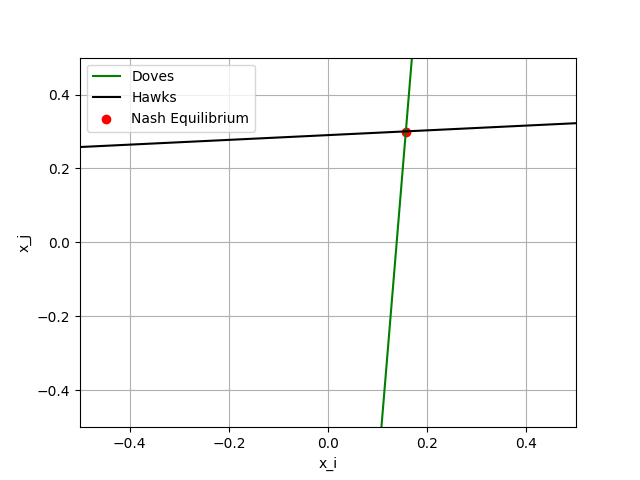
\includegraphics[scale=0.8]{plot.png}
    \caption{Nash equilibrium and best reply function\label{figure1}}
\end{figure}

\section{Rationalizability}

Rationalizability can be defined as a solution concept that is achieved by iteratively eliminating strictly dominated strategies until we reach a set of strategies that are rational to play. This process can be seen as a limit, as we continue to eliminate strictly dominated strategies until no such strategies remain.

Furthermore, rationalizability provides a set of strategies that are considered rational to play in scenarios where it is common knowledge that all agents involved in the game are rational. This means that each agent is aware of the other agents' rationality and acts accordingly. In such scenarios, rationalizability helps identify the strategies that are most likely to be played based on the assumptions of rationality and common knowledge among all agents.

\begin{table}[htbp]
    \centering
    \caption{Rationalizability Learning Steps}
    \label{table1}
    \begin{tabular}{|c|c|c|}
    \hline
    \textbf{Step} & \textbf{Doves} & \textbf{Hawks} \\ \hline
    0             & [-0.5, 0.5]      & [-0.5, 0.5]      \\ 
    1             & [0.10382514, 0.16939891]     & [0.26190476, 0.33333333]     \\ 
    2             & [0.1537861, 0.15846995]     & [0.30503513, 0.30971897]     \\ 
    3             & [0.15661433, 0.15692146]     & [0.30860377, 0.30893833]     \\ 
    4             & [0.15684833, 0.15687027]     & [0.30880579, 0.30882772]     \\ 
    5             & [0.15686158, 0.15686302]     & [0.3088225, 0.30882407]     \\ 
    6             & [0.15686268, 0.15686278]     & [0.30882345, 0.30882355]\\
    7             & [0.15686274, 0.15686275]     & [0.30882352, 0.30882353]\\
    8             & [0.15686274, 0.15686275]     & [0.30882352, 0.30882353]     \\ \hline
    \end{tabular}
    \end{table}

As we can see from the table\ref{table1} the rationalizability converges at the Nash equilibrium in 8 step, due to the
fact 
that we limited the number of significant digits at 8,
 but it's just a way to see the process convergence at $+ \infty$. 
\end{document}